\section{Introduction}
\noindent
In recent years\RE{,} the grow of \RE{potential} business opportunities related to the use of drone technology \RE{have} motivated the appearance of an interesting body of methodological literature on \RE{the optimization} of the use of such technology. 
We can find examples of that in many different sectors, like telecommunication\RE{s} where drones can be adopted in place of traditional infrastructures to provide connectivity (see\RE{,} for example \cite{art:Amorosi2018}, \cite{art:Chiaraviglio2018}, \cite{Jimenez2018}, \cite{art:Amorosi2019}, and \cite{art:Chiaraviglio2019a}), or to temporary deal with the \RE{damage} caused by a disaster (\cite{art:Chiaraviglio2019}), deliveries (see\RE{,} for example \cite{art:Mathew2015} , \cite{art:Ferrandez2016}, \cite{art:Poikonen2020} and \cite{art:Amorosi2020}), also in emergency contexts (\cite{art:Wen2016}), inspection (\cite{art:Trotta2018}) and others.
The reader is referred to the recent surveys \cite{art:Otto2018} and \cite{art:Chung2020} for further details.\\
\noindent
Among the different aspects that can be considered\RE{,} we want to focus, \RE{due to} its relationship to the development in this paper, to the design, coordination and optimization of the combined routes of drones with a base vehicle. After the initial paper \cite{MURRAY201586}, where a combined model of truck and drone is considered, the work \cite{Ulmer2018} also considers another model where trucks and drones are dispatched as \RE{the} order\RE{s} are placed and analyze the effect of different policies for either the truck or the drone. Other papers, as\RE{,} for instance, \cite{art:Campbell2017}, \cite{art:Carlsson2017} and \cite{art:Dayarian2017}, have also considered hybrid truck-and-drone models in order to mitigate the limited delivery range of drones. In \cite{Poikonen2019} the authors advance on the coordination problem considering the \textit{Mothership and drone routing problem} where these two vehicles are used to design a route that visits a number of points allowing the truck to launch and recover the drone in a continuous space. More recently, in \cite{art:Poikonen2020}, the authors consider the \textit{$k$-Multi-Visit drone routing problem} where a truck that acts as a mobile depot only allowed to stop in a predefined set of points, launches drones that can deliver more than one package to their designated destination points. %\CV{There are some references where we mention the authors, and other not}
\noindent
Many of these papers make \RE{assumptions} that the set of allowable locations to launch/retrieve a drone are fixed and known a priori, the \CV{operations} performed by the drone consist of delivering to a single point and the coordination is between a truck and a single drone. These assumptions may be appropriate in some frameworks\RE{,} but, in other cases, it may be better to relax them.\\
\noindent
In particular, only \RE{a} few papers in \RE{the} literature focus on \RE{drone} operations consisting \RE{of} traversing graphs rather than visiting single points. Later authors in 
\cite{art:Campbell2018} introduce the \textit{Drone Rural Postman Problem} (DRPP). \RE{Those} authors present a solution algorithm based on the approximation of curves in the plane by polygonal chains \CV{that iteratively} increases the number of points in the polygonal chain where the UAV can enter or leave. Thus, they solve the problem as a discrete optimization problem trying to better define the curve by increasing the number of points. The authors consider also the case in which the drone has limited \RE{endurance} and thus it cannot serve all the lines. To deal with this latter case, they assume to have a fleet of drones and the problem consists in finding a set of routes, each of limited length.\\
In \cite{art:CAMPBELL202160}  this problem has been defined as the \textit{Length Constrained K-drones Rural Postman Problem}, a continuous optimization problem where a fleet of homogeneous drones have to jointly service (traverse) a set of (curved or straight) lines of a network. The authors design and implement a branch-and-cut algorithm for its solution and a matheuristic algorithm capable of providing good solutions for large\RE{-}scale instances of the problem.\\
Scanning the literature of arc routing problems involving hybrid systems consisting \RE{of} one vehicle and one or multiple drones, the number of contributions is rather limited.\\
In \cite{art:Tokekar2016} the authors study the path planning problem of a system composed of a ground robot and one drone in precision agriculture and solve it by applying orienteering algorithms. \RE{Moreover,} the paper \cite{art:Garone2010} studies the problem of \RE{path} planning for systems consisting \RE{of} a carrier vehicle and a carried one to visit a set of target points and assuming that the carrier vehicle moves in the continuous space.\\
To the best of our knowledge, \RE{the paper \cite{art:Amorosi2021} is the only one} that deals with the coordination of a mothership with one drone to visit targets represented by graphs. The authors made different assumptions on the route followed by the mothership: it can move on a continuous framework (the Euclidean plane), ii) on a connected piecewise linear polygonal chain\RE{,} or iii) on a general graph. In all cases, the authors develop exact formulations resorting to mixed integer second\RE{-}order cone programs and propose a matheuristic algorithm capable to obtain high quality solutions in short computing time.
\\
In this paper we deal with an extension of the problem studied in \cite{art:Amorosi2021} for which we propose a novel truck-and-multi-\RE{drone} coordination model. We consider a system where a base vehicle (mothership) \RE{travels} in \JP{the} continuous space and has to support the launch/retrieve of a number of drones that must visit graphs. \RE{Our} contribution \RE{over} the existing literature is to extend the coordination beyond a single drone to the more cumbersome case of several drones and operations to traversing graphs rather than visiting single points. 
\noindent
\JP{In particular, we focus on two different versions. In the first one, called \textit{complete overlapping model}, operations consisting on the launching and retrieving of a set of drones are done sequentially so that no two consecutive launching are  possible without retrieving the previously launched drones (See Figure \ref{fig:2-models} left).  The second version, called \textit{partial overlapping model}, allows consecutive launching or retrieving actions so that the visits of several drones to their target graphs are allowed to partially overlap over the time (See Figure \ref{fig:2-models} right). In both cases, we present  mathematical programming formulations, valid inequalities to strengthen them and ad hoc matheuristics to deal with large sized instances of the problem.\\}
\noindent

% \pgfplotsset{compat=1.15}
\usetikzlibrary{arrows}
\begin{figure}[h!]
\centering
\definecolor{ffwwzz}{rgb}{1,0.4,0.6}
\definecolor{ffqqqq}{rgb}{1,0,0}
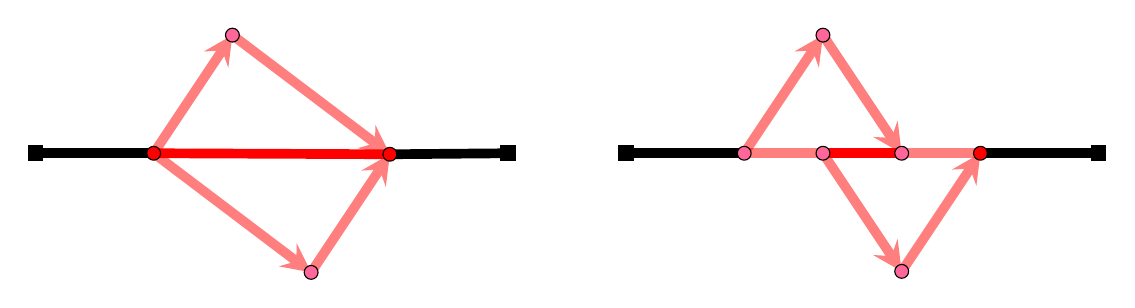
\begin{tikzpicture}[line cap=round,line join=round,>=triangle 45,x=0.5cm,y=0.5cm]
\fill[line width=2pt,fill=black] (3.8,5.2) -- (4.2,5.2) -- (4.2,4.8) -- (3.8,4.8) -- cycle;
\fill[line width=2pt,fill=black] (15.8,5.2) -- (16.2,5.2) -- (16.2,4.8) -- (15.8,4.8) -- cycle;
\fill[line width=2pt,fill=black] (18.8,5.2) -- (19.2,5.2) -- (19.2,4.8) -- (18.8,4.8) -- cycle;
\fill[line width=2pt,fill=black] (30.8,5.2) -- (31.2,5.2) -- (31.2,4.8) -- (30.8,4.8) -- cycle;
\draw [line width=3.5pt] (4,5)-- (7,5);
\begin{scope}[transparency group, opacity=0.5]
\draw [-stealth,line width=3.5pt,color=ffqqqq] (7,5) -- (9,8);
\draw [-stealth,line width=3.5pt,color=ffqqqq] (7,5) -- (11,1.974194108172913);
\draw [-stealth,line width=3.5pt,color=ffqqqq] (9,8) -- (13,4.974194108172913);
\draw [-stealth,line width=3.5pt,color=ffqqqq] (11,1.974194108172913) -- (13,4.974194108172913);
\end{scope}
\draw [line width=3.5pt,color=ffqqqq] (7,5)-- (13,4.974194108172913);
\draw [line width=3.5pt] (13,4.974194108172913)-- (16,5);
\draw [line width=3.5pt] (19,5)-- (22,5);
\draw [line width=3.5pt] (28,5)-- (31,5);
\begin{scope}[transparency group, opacity=0.5]
\draw[-stealth,line width=3.5pt, red] (22,5) -- (24,8);
\draw[-stealth,line width=3.5pt, red] (24,8) -- (26,5);
\draw[-stealth,line width=3.5pt, red] (24,5) -- (26,2);
\draw[-stealth,line width=3.5pt, red] (26,2) -- (28,5);
\end{scope}
\draw [line width=3.5pt,color=ffqqqq] (24,5)-- (26,5);
\draw [line width=3.5pt,color=ffqqqq, opacity=0.5] (22,5)-- (24,5);
\draw [line width=3.5pt,color=ffqqqq, opacity=0.5] (26,5)-- (28,5);
\begin{scriptsize}
\draw [fill=ffqqqq] (7,5) circle (2.5pt);
\draw [fill=ffwwzz] (9,8) circle (2.5pt);
\draw [fill=ffwwzz] (11,1.974194108172913) circle (2.5pt);
\draw [fill=ffqqqq] (13,4.974194108172913) circle (2.5pt);
\draw [fill=ffwwzz] (22,5) circle (2.5pt);
\draw [fill=ffqqqq] (28,5) circle (2.5pt);
\draw [fill=ffwwzz] (24,8) circle (2.5pt);
\draw [fill=ffwwzz] (26,2) circle (2.5pt);
\draw [fill=ffwwzz] (26,5) circle (2.5pt);
\draw [fill=ffwwzz] (24,5) circle (2.5pt);
\end{scriptsize}
\end{tikzpicture}
\caption{Models with complete and partial overlapping.\label{fig:2-models}}
\end{figure}
\noindent
\JP{The work is structured as follows: Section \ref{section:desc} provides a detailed description of the problem under consideration. Section \ref{Form}  develops valid mixed integer nonlinear programming formulations for the two versions of the considered problem. Here, we also show the relationship between the two models and prove that the second model is a relaxation of the first one. Section \ref{bounds} provides some valid inequalities that strengthen the formulations and derives upper and lower bounds on the bigM constants introduced in the proposed formulations. Section \ref{Math} presents details of the matheuristic algorithms designed to handle large sized instances. In Section \ref{section:results} we report the results obtained testing the formulations and the matheuristic algorithm on different classes of planar graphs to assess its effectiveness. In Section \ref{section:CS}, we introduce an illustrative example applying the coordination models to the Courtyards Festival of Cordoba. Section \ref{section:CR} concludes the paper. Finally, for the sake of completeness, we have included an appendix with an extension of the model of complete overlapping where the drones are not assumed to be homogeneous. %\CV{We present a mixed integer second order cone programming formulation, develop several valid inequalities to strengthen it and report computational results assessing its performance.} 
}